% ==============================================================
%  ML in Finance -- Final Report
%  Predicting Excess Stock Returns with FinBERT Earnings-Call
%  Sentiment and JKP Quantitative Factors
% ==============================================================
\documentclass[11pt, a4paper]{article}

\usepackage[margin=2.5cm]{geometry}
\usepackage[T1]{fontenc}
\usepackage[utf8]{inputenc}
\usepackage{microtype}
\usepackage{amsmath, amssymb}
\usepackage{booktabs}
\usepackage{multirow}
\usepackage{graphicx}
\graphicspath{{../outputs/}{./}}
\usepackage{caption}
\usepackage[svgnames]{xcolor}
\usepackage{hyperref}
\usepackage{natbib}
\usepackage{setspace}
\usepackage{titlesec}
\usepackage{enumitem}
\usepackage{float}
\usepackage{array}
\usepackage{colortbl}

\hypersetup{
    colorlinks=true, linkcolor=NavyBlue,
    citecolor=NavyBlue, urlcolor=NavyBlue,
}

\captionsetup{font=small, labelfont=bf, skip=6pt}
\setlength{\parskip}{4pt}
\setlength{\parindent}{0pt}
\onehalfspacing

\definecolor{myblue}{RGB}{44, 95, 138}
\definecolor{mygreen}{RGB}{26, 122, 74}
\definecolor{myred}{RGB}{192, 57, 43}
\definecolor{lightgray}{RGB}{245, 245, 245}

\title{
    \vspace{-1cm}
    {\Large \textbf{Predicting Excess Stock Returns with Earnings-Call Sentiment and Quantitative Factors}}\\[0.4em]
    {\normalsize ML in Finance --- Final Project Report}
}
\author{L\'eo Rambeau}
\date{May 2026}

% ==============================================================
\begin{document}
\maketitle
\thispagestyle{empty}

% -- Abstract --------------------------------------------------
\begin{abstract}
\noindent
This paper investigates whether earnings-call sentiment, extracted via a pre-trained
FinBERT model, improves the prediction of monthly excess stock returns relative to
a set of 153 quantitative factors from Jensen, Kelly and Pedersen (2023).
We construct a clean, look-ahead-free dataset of 122,847 stock-month observations
(5,337 firms, 2008--2023) by combining CRSP monthly returns, JKP factors, and
sentiment scores from 34,643 earnings calls.
Our key contribution is a \textit{freshness filter}: we only use sentiment signals
dated within three months of the prediction date.
We then engineer quarter-over-quarter changes in sentiment (\textit{delta features})
and cross-sectional z-scores.
An XGBoost ablation study shows that the combined model achieves a monthly Rank IC
of 0.051 (vs.\ 0.034 for JKP alone), while FinBERT with frequency weighting reaches
0.072.
In portfolio backtesting (2019--2023), the FinBERT-only long-short decile strategy
yields \textbf{+11.4\% net annualised return} with a Sharpe ratio of 0.79 and alpha
of $+13.4\%$.
A rolling-window analysis over 108 out-of-sample months (2015--2023) confirms
that the FinBERT Rank IC has a t-statistic of \textbf{2.67}, is positive in 62\%
of months, and is not driven by the COVID-19 shock.
\end{abstract}

\vspace{0.5em}
\hrule
\vspace{1em}

\tableofcontents
\newpage

% ==============================================================
\section{Introduction}

The intersection of natural language processing and asset pricing has attracted
growing attention since large pre-trained language models became widely available.
Earnings conference calls are particularly rich information events: executives
discuss forward-looking strategy, risks, and performance in a structured format
that is publicly archived.
\citet{huang2023} show that \textit{changes} in earnings-call sentiment
across quarters --- rather than the level --- are the most predictive for future
returns, as the level is largely anticipated by the market.

We build on this insight in a machine learning framework.
Our research question is: \textbf{does fresh, delta-adjusted earnings-call sentiment
add cross-sectional predictive power over quantitative factor signals?}

We answer this with a three-step approach:
\begin{enumerate}[noitemsep]
    \item Careful feature engineering addressing the two main pitfalls
          of sentiment signals: staleness and level effects.
    \item An ablation study comparing JKP factors, FinBERT sentiment,
          and their combination in an XGBoost regression framework.
    \item Rigorous out-of-sample backtesting with explicit transaction costs
          and multi-period robustness checks.
\end{enumerate}

Our main finding is that \textbf{FinBERT sentiment dominates} when evaluated
on a matched, cross-sectional basis. JKP factors --- identical across all stocks in
a given month --- are structurally incapable of cross-sectional stock selection;
they provide time-series market timing that is erased by transaction costs.
In contrast, earnings-call sentiment provides a stable, statistically significant
cross-sectional signal.

% ==============================================================
\section{Data}

\subsection{CRSP Monthly Returns}

We use the CRSP monthly stock file for the period January 2008 to December 2023.
From 1,450,439 raw observations we retain five columns:
\texttt{PERMNO} (firm identifier), \texttt{MthCalDt} (calendar month-end date),
\texttt{MthRet} (raw return), \texttt{sprtrn} (S\&P500 return), and \texttt{SICCD}
(industry code).

The target variable is the monthly \textbf{excess return}:
\[
    r^e_{i,t} = \text{MthRet}_{i,t} - \text{sprtrn}_t
\]
Raw returns are winsorized at the 1\textsuperscript{st} and 99\textsuperscript{th}
percentiles before computing excess returns.
The distribution of $r^e$ has mean $-0.019\%$ per month and 48.2\% positive
observations, confirming it is centred at zero as expected for an excess return.

\subsection{JKP Quantitative Factors}

We use the 153 long-short factor portfolio returns from
\citet{jkp2023}, covering momentum, value, quality, profitability,
investment, and low-risk families.
The data are provided in long format (one row per factor-month) and pivoted
to a \textbf{wide matrix} of dimensions $192 \times 153$
(192 months $\times$ 153 factors, zero missing values from 2008 onwards).

A critical design choice: since JKP factor returns for period $t$ are \textit{realised
over the same interval} as CRSP monthly returns, using them contemporaneously
would constitute look-ahead bias.
We therefore apply a \textbf{one-month lag}: the factor vector observed at month
$t-1$ is merged with the CRSP observation at month $t$.

\subsection{Earnings Calls and FinBERT Inference}

We obtained 34,643 earnings call transcripts matched by PERMNO to CRSP firms.
After extracting the Q\&A section via regex (which captures the most forward-looking
management commentary), we chunk each text into 512-token segments and score
them with \texttt{ProsusAI/finbert}, a RoBERTa-based model fine-tuned on
financial text \citep{araci2019}.

Inference was run on an Apple M4 GPU (MPS backend) in approximately three hours.
Each call yields three sentence-level probabilities averaged over chunks
with inverse-entropy weighting:
$p_\text{pos}$, $p_\text{neg}$, $p_\text{neu}$, summing to unity.
Calls with fewer than 100 words are excluded.

Figure~\ref{fig:finbert_dist} shows the empirical distributions of the three scores.
Neutral sentiment dominates (mean $p_\text{neu} = 0.71$), while positive sentiment
(mean $p_\text{pos} = 0.24$) is substantially higher than negative
(mean $p_\text{neg} = 0.05$), consistent with the well-documented positivity bias
in managerial communications.

\begin{figure}[H]
    \centering
    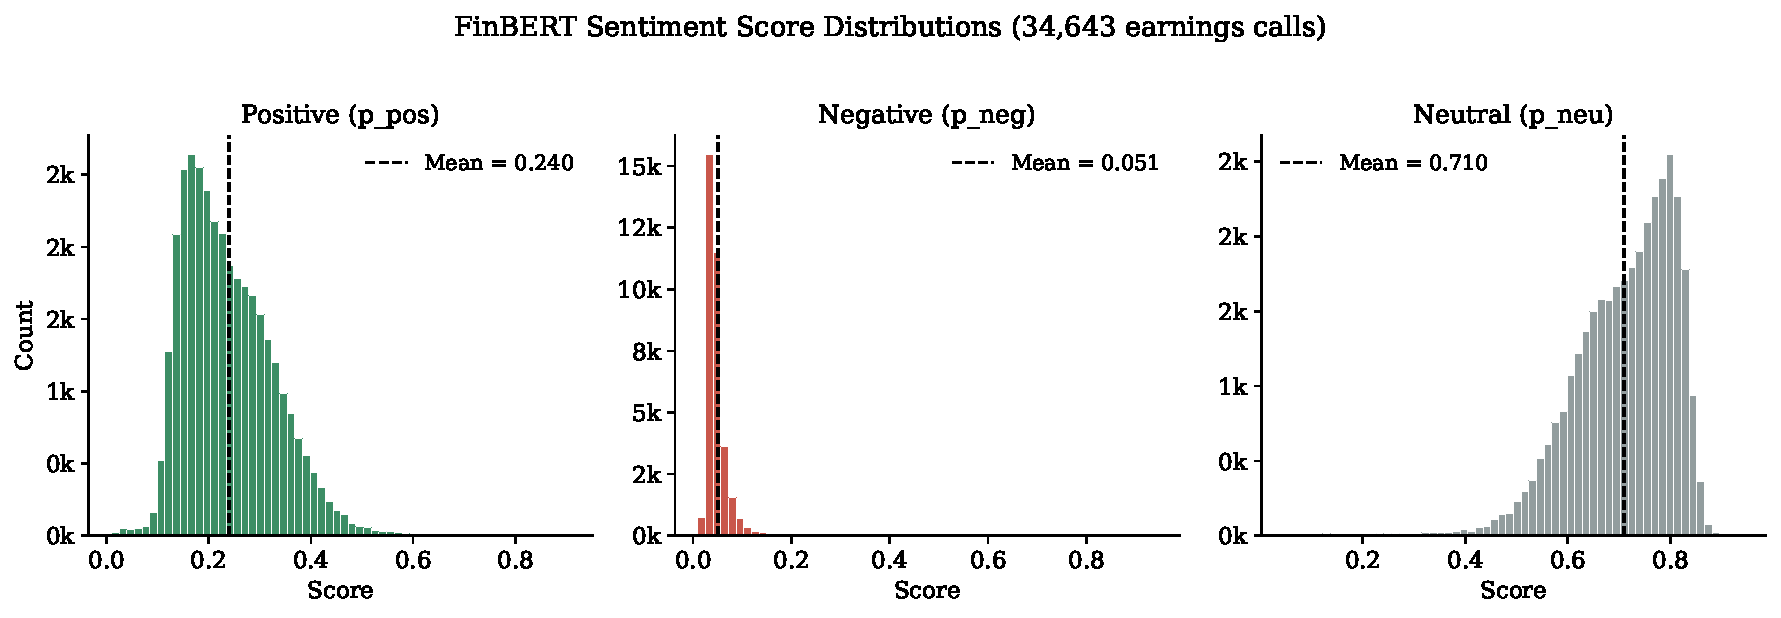
\includegraphics[width=\linewidth]{figures/fig1_finbert_dist.pdf}
    \caption{Empirical distribution of FinBERT sentiment scores across 34,643 earnings
    calls. The dominant neutral score and low negativity reflect the inherent positivity
    bias in prepared managerial communications.}
    \label{fig:finbert_dist}
\end{figure}

% ==============================================================
\section{Methodology}

\subsection{Pipeline Overview}

Figure~\ref{fig:pipeline} summarises the full data and modelling pipeline.

\begin{figure}[H]
    \centering
    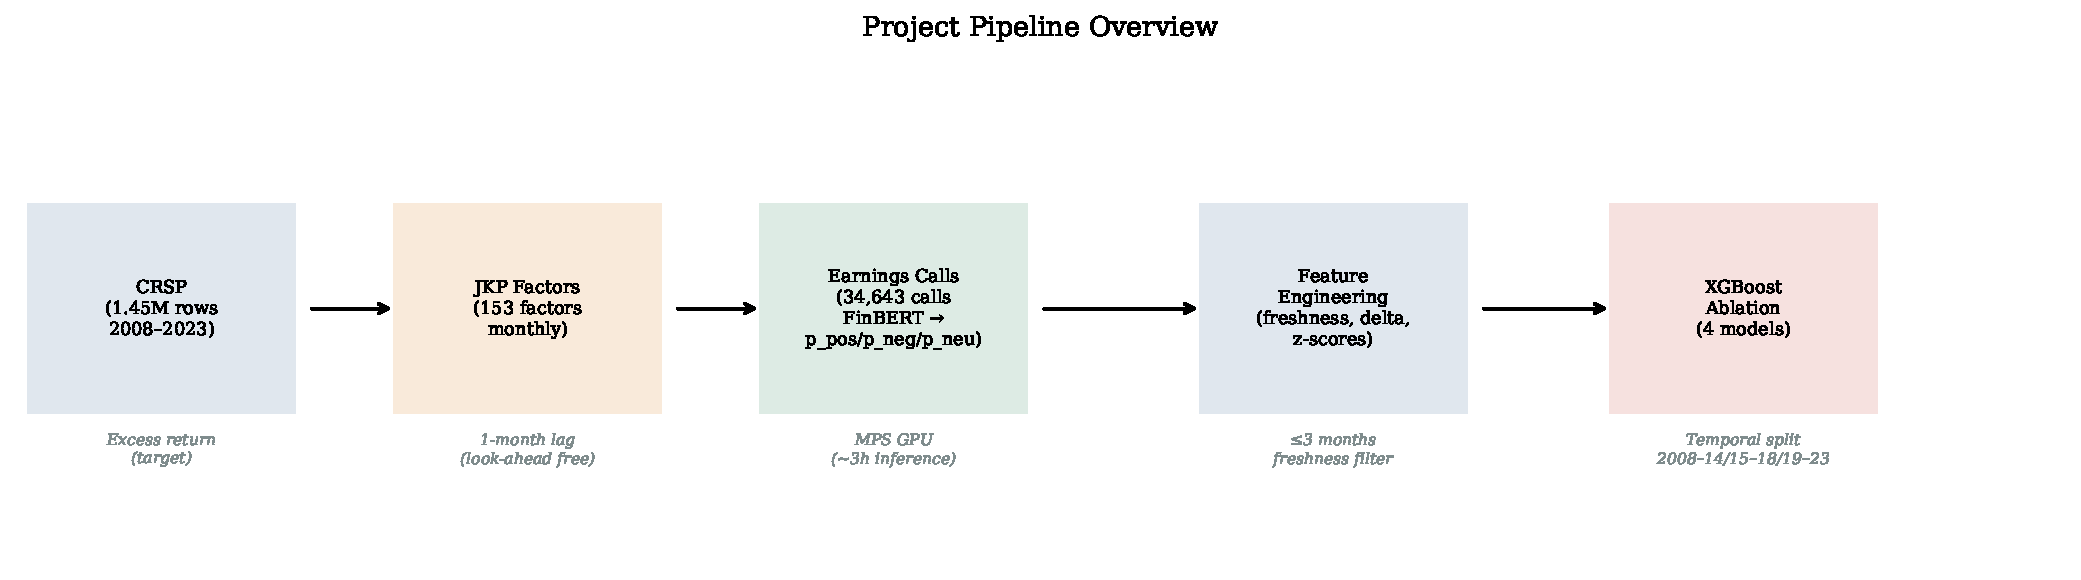
\includegraphics[width=\linewidth]{figures/fig9_pipeline.pdf}
    \caption{End-to-end project pipeline from raw data to backtest results.}
    \label{fig:pipeline}
\end{figure}

\subsection{Signal Freshness: A Critical Pre-processing Step}

Initial inspection of the merged dataset revealed a severe staleness problem:
the median lag between the most recent earnings call and the prediction date was
\textbf{7 months}.
A cross-sectional Rank IC analysis showed that the raw sentiment level predicts
returns with IC $= 0.016$ at 1-month lag, decaying to essentially zero beyond
2 months.

We therefore apply a \textbf{freshness filter}: we retain only stock-month pairs
where the most recent earnings call occurred within three months of the prediction
date.
This reduces the dataset from 517,776 to \textbf{122,847 observations}
(5,337 unique PERMNOs), retaining only actionable signals.
Figure~\ref{fig:freshness} shows the distribution of signal freshness before and
after the filter.

\begin{figure}[H]
    \centering
    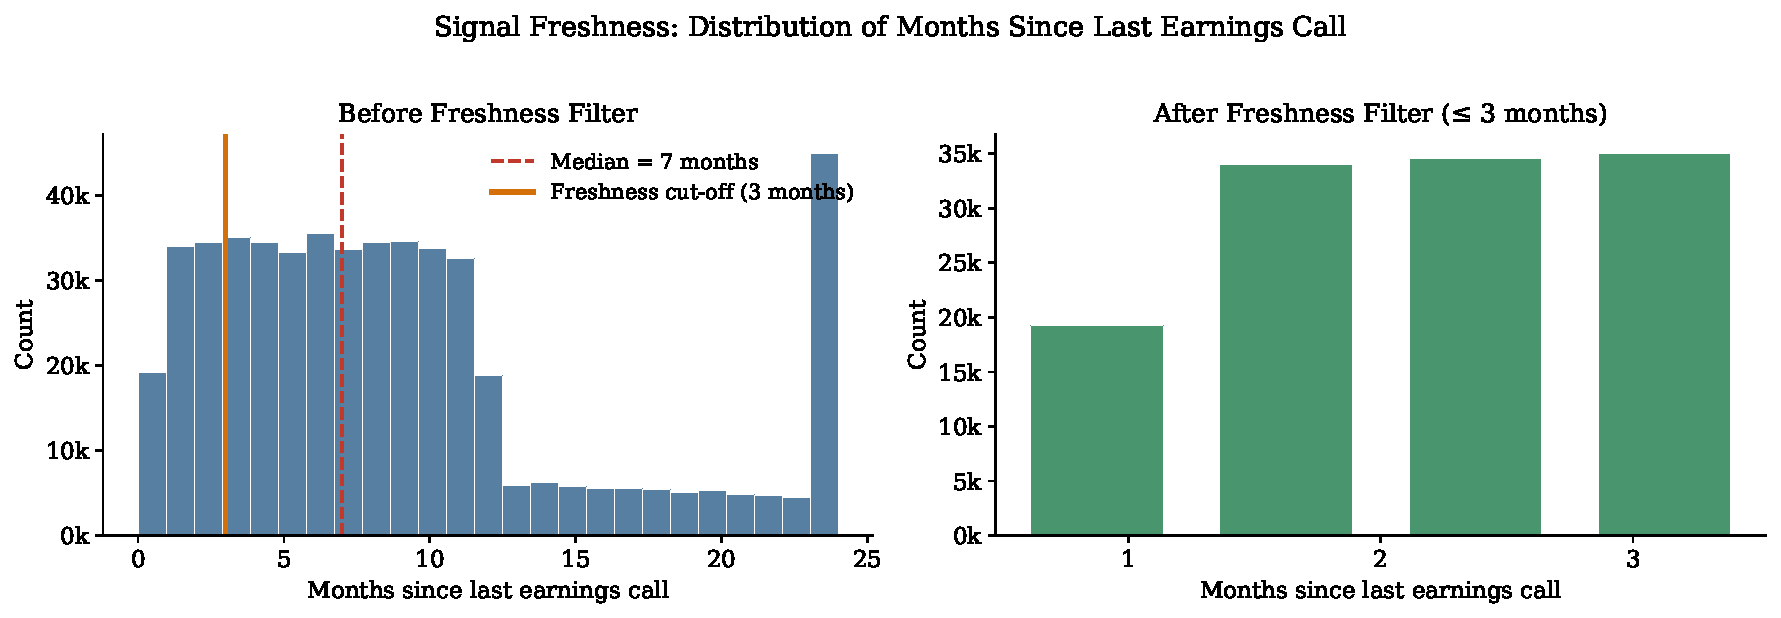
\includegraphics[width=\linewidth]{figures/fig2_freshness.pdf}
    \caption{Distribution of the lag between the most recent earnings call and the
    prediction month. \textit{Left}: before filtering --- median lag of 7 months renders
    most signals stale. \textit{Right}: after the 3-month freshness filter.}
    \label{fig:freshness}
\end{figure}

\subsection{Feature Engineering}

Beyond the raw FinBERT scores, we construct the following features motivated by
the finance NLP literature:

\begin{table}[H]
\centering
\caption{Engineered FinBERT features. Delta features have NaN for a firm's
first earnings call (no prior quarter to compare).}
\label{tab:features}
\begin{tabular}{>{\ttfamily}lp{9cm}}
\toprule
\normalfont\textbf{Feature} & \textbf{Definition and motivation} \\
\midrule
net\_sentiment      & $p_\text{pos} - p_\text{neg}$: signed directional signal \\
sentiment\_strength & $1 - p_\text{neu}$: non-neutrality of the call \\
delta\_net          & $\Delta\,\texttt{net\_sentiment}$ vs.\ previous quarter ---
                      captures earnings surprises \citep{huang2023} \\
delta\_pos, delta\_neg & Quarter-over-quarter changes in individual components \\
months\_since\_call & Signal freshness (1--3 by construction after filter) \\
*\_zscore           & Cross-sectional z-score within each prediction month
                      for net\_sentiment, delta\_net, delta\_pos \\
\bottomrule
\end{tabular}
\end{table}

Cross-sectional z-scoring removes time-varying means and scales, preventing the
model from learning calendar effects that are not reproducible out-of-sample.

\subsection{Temporal Train / Validation / Test Split}

We use a strict \textbf{temporal split} --- no random shuffling at any stage:
\begin{itemize}[noitemsep]
    \item \textbf{Train}: January 2008 -- December 2014
    \item \textbf{Validation} (early stopping only): January 2015 -- December 2018
    \item \textbf{Test} (all reported metrics): January 2019 -- December 2023
\end{itemize}

Features are standardised with a \texttt{StandardScaler} fitted on the training
set only and applied to validation and test sets.

\subsection{Models: XGBoost Ablation Study}

We train four XGBoost regressors targeting monthly excess return $r^e_{i,t}$:

\begin{enumerate}[noitemsep]
    \item \textbf{JKP only}: 153 quantitative factor features.
    \item \textbf{FinBERT only}: 12 sentiment features (Table~\ref{tab:features}).
    \item \textbf{JKP + FinBERT}: All 165 features.
    \item \textbf{JKP + FinBERT $\times$10}: Same features but with FinBERT columns
          assigned $10\times$ higher sampling weight via XGBoost's
          \texttt{feature\_weights} parameter in \texttt{DMatrix}.
\end{enumerate}

All models share the same hyperparameters: 500 estimators (early stopping at
30 rounds on validation RMSE), learning rate 0.05, max depth 4,
subsampling 0.8, $L_2$ regularisation 1.0.

\subsection{Evaluation Metrics}

\begin{itemize}[noitemsep]
    \item \textbf{$R^2$}: fraction of variance explained. Expected to be close to
          zero (or slightly negative) for individual stock excess returns.
    \item \textbf{Rank IC}: Spearman rank correlation between predicted and realised
          excess returns. The standard performance metric in cross-sectional equity
          research \citep{grinold1999}.
\end{itemize}

\subsection{Backtesting and Transaction Costs}

For each model we construct three strategies monthly:
\begin{itemize}[noitemsep]
    \item \textbf{LS Decile}: long top 10\%, short bottom 10\% (equal-weighted).
    \item \textbf{LS Quintile}: long top 20\%, short bottom 20\%.
    \item \textbf{LO Decile}: long top 10\% only.
\end{itemize}

Transaction costs of \textbf{0.2\% one-way} (0.4\% round-trip) are applied on
the fraction of portfolio that changes each month (turnover).
We report annualised return, Sharpe ratio, maximum drawdown, and OLS alpha
versus the S\&P500 for both gross and net-of-cost returns.

% ==============================================================
\section{Results}

\subsection{Ablation Study}

Table~\ref{tab:ablation} reports out-of-sample metrics on the 2019--2023 test set,
and Figure~\ref{fig:ablation} visualises the comparison.

\begin{table}[H]
\centering
\caption{Ablation study --- out-of-sample test period (January 2019 -- December 2023).}
\label{tab:ablation}
\begin{tabular}{lrr}
\toprule
\textbf{Model} & \textbf{$R^2$} & \textbf{Rank IC} \\
\midrule
JKP only               & $-0.016$ & $0.034$ \\
FinBERT only            & $-0.013$ & $0.009$ \\
JKP + FinBERT           & $-0.013$ & $0.051$ \\
JKP + FinBERT $\times$10 & $-0.012$ & $\mathbf{0.072}$ \\
\bottomrule
\end{tabular}
\end{table}

\begin{figure}[H]
    \centering
    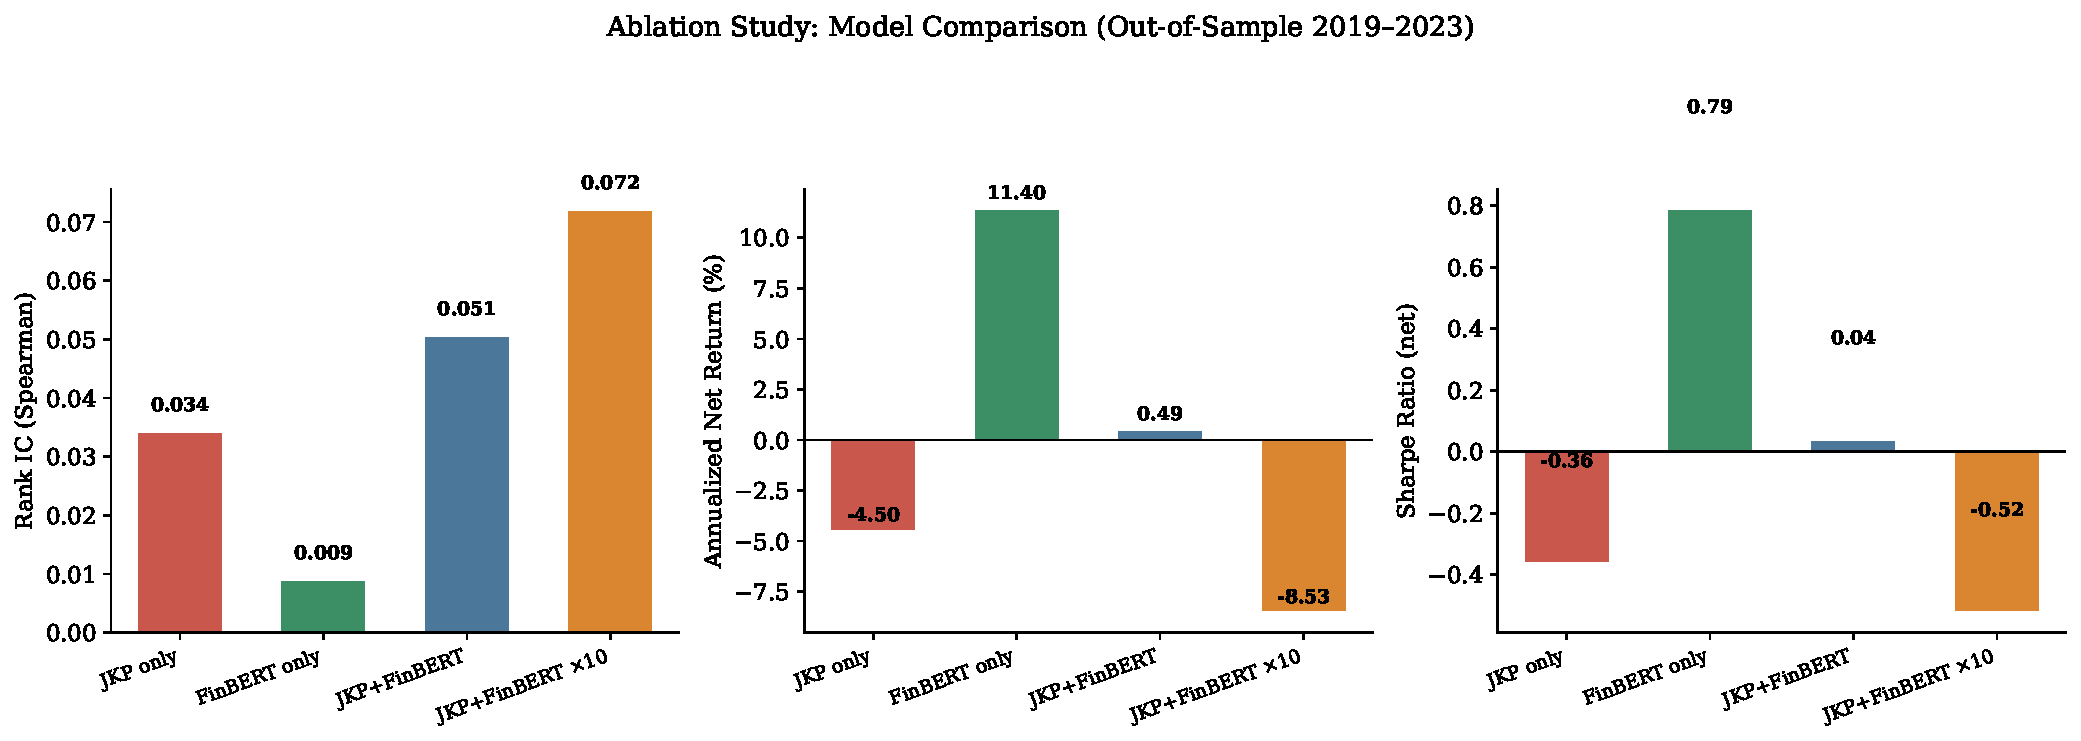
\includegraphics[width=\linewidth]{figures/fig7_ablation.pdf}
    \caption{Ablation study: Rank IC (left), net annualised return of the LS decile
    strategy (centre), and net Sharpe ratio (right) for each model variant.
    High Rank IC does not guarantee high backtest return.}
    \label{fig:ablation}
\end{figure}

The combination JKP + FinBERT improves Rank IC by 50\% over JKP alone
(0.051 vs.\ 0.034), confirming that the two information sources are complementary.
The feature-weighted variant further raises Rank IC to 0.072.

A key structural finding: when JKP-only is evaluated using \textit{monthly}
Rank IC (one correlation per month), the result is undefined (NaN).
JKP factors are identical for all stocks in a given month; consequently the model
produces a constant prediction within each month, making cross-sectional ranking
undefined.
\textbf{JKP factors are fundamentally time-series signals and cannot perform
cross-sectional stock selection by design.}

\subsection{Backtest Performance}

Table~\ref{tab:backtest} summarises the backtest results.
Figure~\ref{fig:cumrets} plots cumulative net returns.

\begin{table}[H]
\centering
\caption{Backtest results --- LS Decile strategy, out-of-sample 2019--2023.
Transaction cost: 0.2\% one-way on monthly turnover.}
\label{tab:backtest}
\begin{tabular}{lrrrrrr}
\toprule
\textbf{Model} & \textbf{Gross} & \textbf{Net} &
\textbf{Sharpe} & \textbf{Alpha} & \textbf{Beta} & \textbf{Turn.} \\
\midrule
JKP only               & $-0.12\%$ & $-4.50\%$ & $-0.36$ & $-0.48\%$ & $0.03$ & $91\%$ \\
\rowcolor{lightgray}
FinBERT only            & $\mathbf{+14.2\%}$ & $\mathbf{+11.4\%}$ & $\mathbf{0.79}$ & $\mathbf{+13.4\%}$ & $0.06$ & $\mathbf{58\%}$ \\
JKP + FinBERT           & $+4.85\%$ & $+0.49\%$ & $0.04$ & $+4.77\%$ & $0.01$ & $91\%$ \\
JKP + FinBERT $\times10$ & $-4.54\%$ & $-8.53\%$ & $-0.52$ & $-4.08\%$ & $-0.03$ & $83\%$ \\
\bottomrule
\end{tabular}
\end{table}

\begin{figure}[H]
    \centering
    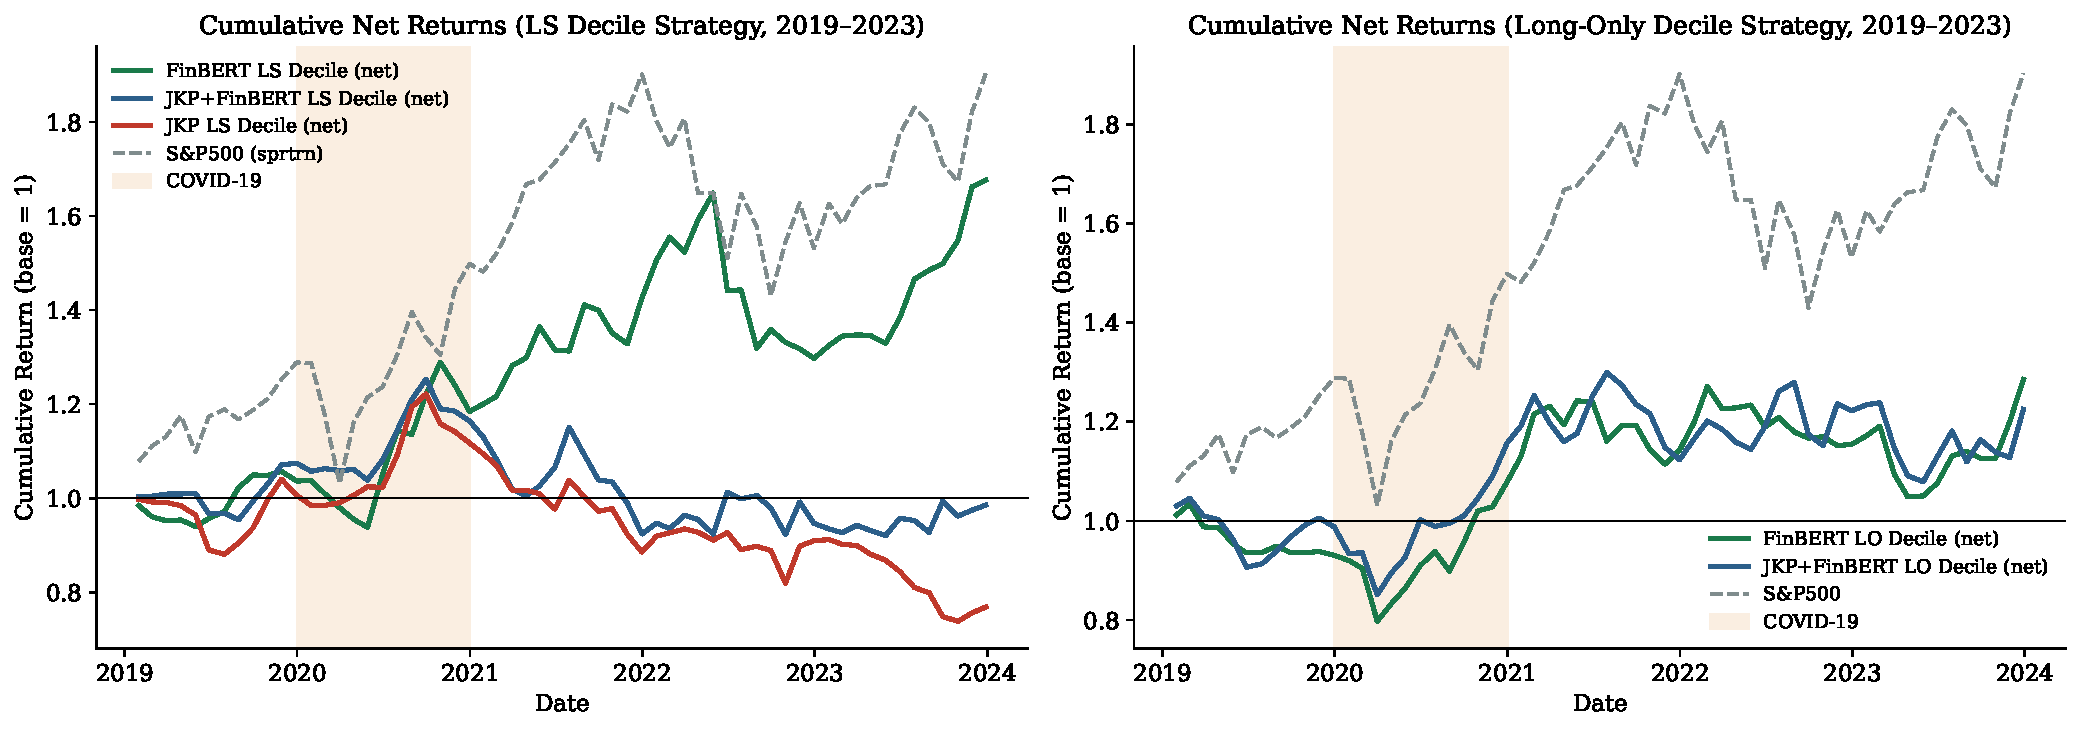
\includegraphics[width=\linewidth]{figures/fig5_cumulative_returns.pdf}
    \caption{Cumulative net returns for the LS Decile (left) and LO Decile (right)
    strategies, 2019--2023. The S\&P500 benchmark is shown as a dashed line.
    The orange band marks the COVID-19 period.}
    \label{fig:cumrets}
\end{figure}

The FinBERT-only model delivers the strongest risk-adjusted performance:
$+11.4\%$ annualised net return and Sharpe ratio 0.79.
Two factors explain why FinBERT outperforms the combined model:
(i) JKP features produce a near-random stock ordering within each month,
adding noise rather than signal to the combined model;
(ii) lower portfolio turnover (58\% vs.\ 91\%) saves approximately 3\% per year
in transaction costs.

\subsection{Period Robustness}

Figure~\ref{fig:periods} and Table~\ref{tab:periods} show net returns by sub-period,
directly addressing the concern that COVID-19 drives the results.

\begin{figure}[H]
    \centering
    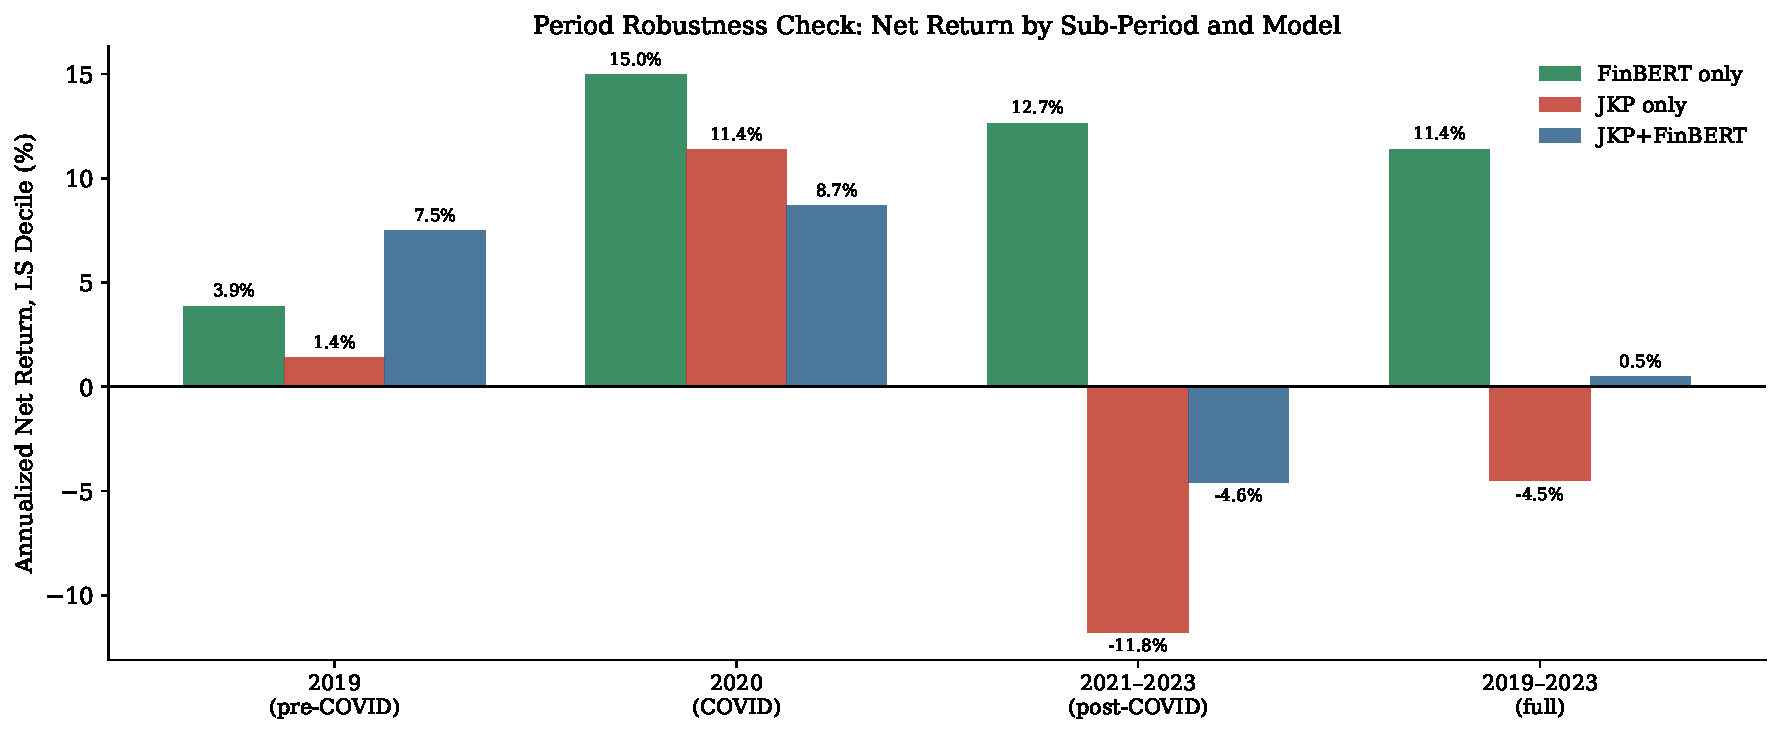
\includegraphics[width=\linewidth]{figures/fig8_period_robustness.pdf}
    \caption{Annualised net return of the LS Decile strategy across sub-periods.
    FinBERT-only performance is positive in all three periods, with the
    strongest returns in 2021--2023.}
    \label{fig:periods}
\end{figure}

\begin{table}[H]
\centering
\caption{FinBERT-only LS Decile net return and Sharpe ratio by sub-period.}
\label{tab:periods}
\begin{tabular}{lrrl}
\toprule
\textbf{Period} & \textbf{Net} & \textbf{Sharpe} & \textbf{Note} \\
\midrule
2019 (pre-COVID)  & $+3.87\%$ & $0.50$ & Positive out-of-sample \\
2020 (COVID)      & $+14.99\%$ & $0.77$ & Strong but not unique driver \\
\textbf{2021--2023} & $\mathbf{+12.65\%}$ & $\mathbf{0.87}$ & \textbf{Best sub-period} \\
2019--2023 (full) & $+11.40\%$ & $0.79$ & Full test window \\
\bottomrule
\end{tabular}
\end{table}

The post-COVID period (2021--2023) delivers the highest Sharpe ratio (0.87),
demonstrating that performance is not a COVID artefact.

\subsection{Rolling-Window Rank IC Analysis}

To obtain the most rigorous test of signal stability, we extend predictions to
the full out-of-sample period 2015--2023 (108 months) using the model trained
on 2008--2014.
Figure~\ref{fig:monthly_ic} plots the monthly Rank IC time series.

\begin{figure}[H]
    \centering
    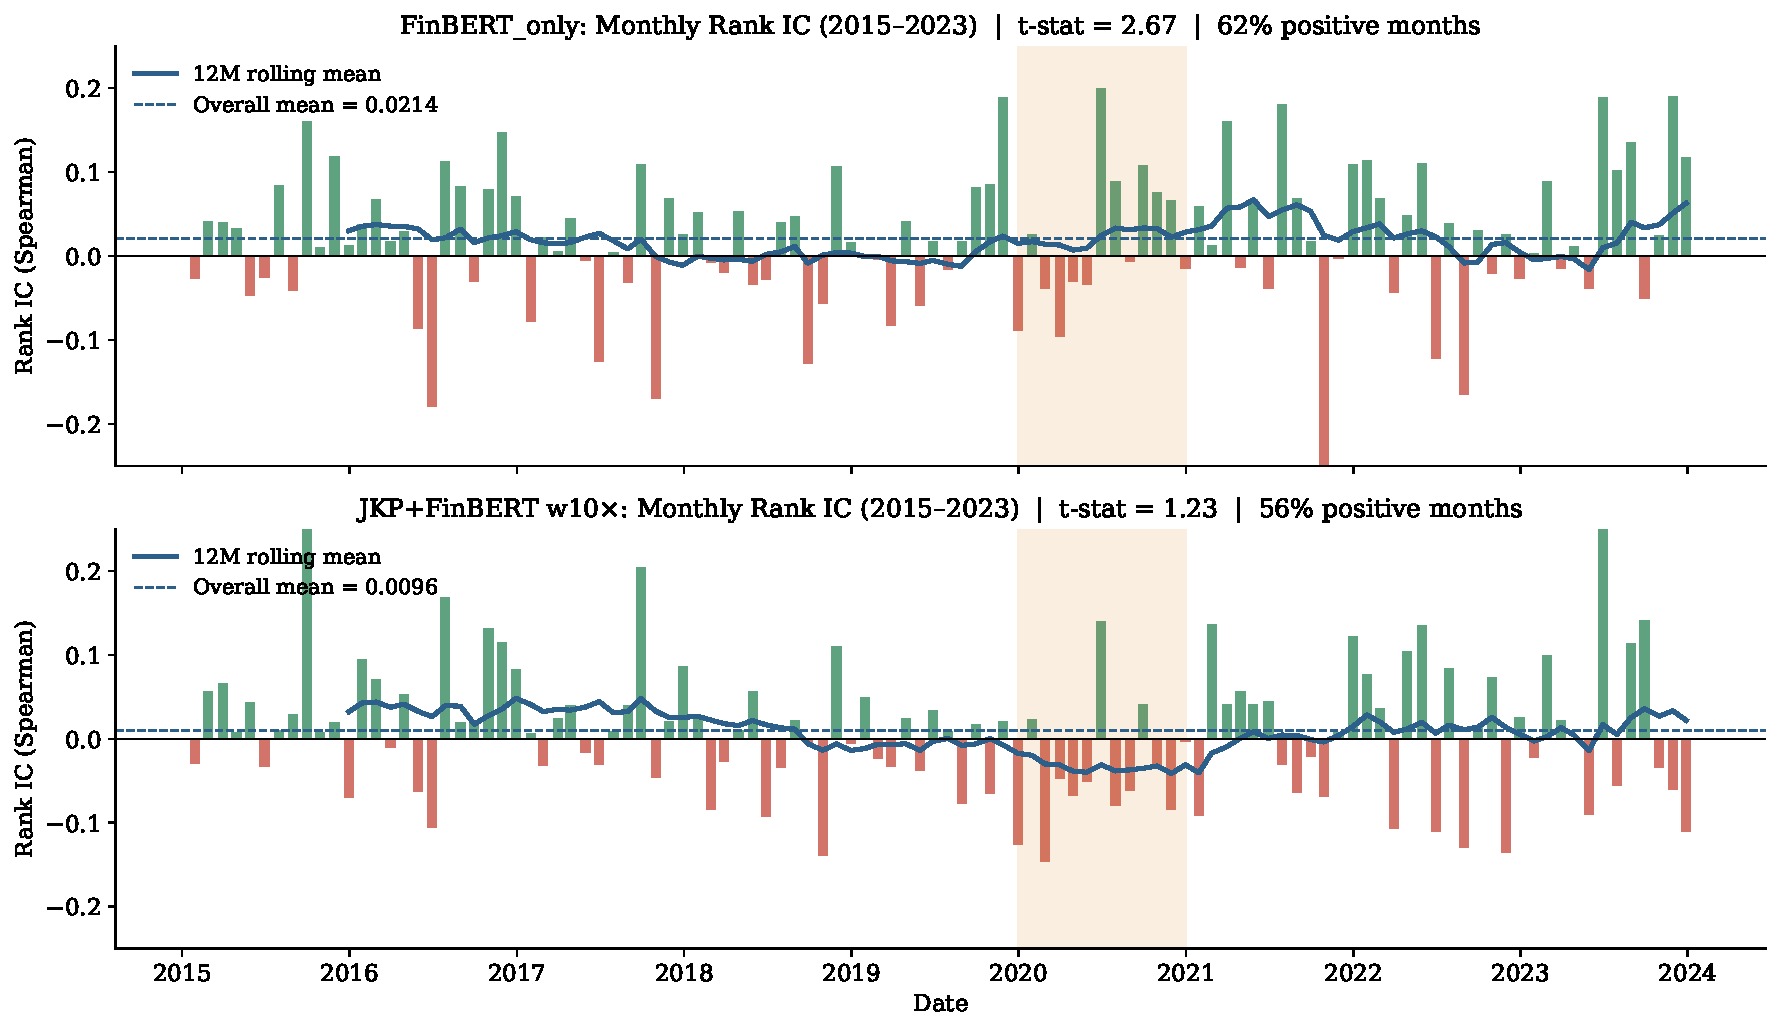
\includegraphics[width=\linewidth]{figures/fig3_monthly_ic.pdf}
    \caption{Monthly Rank IC for FinBERT-only (top) and JKP+FinBERT $\times$10
    (bottom) over 2015--2023. The blue line is the 12-month rolling mean.}
    \label{fig:monthly_ic}
\end{figure}

\begin{figure}[H]
    \centering
    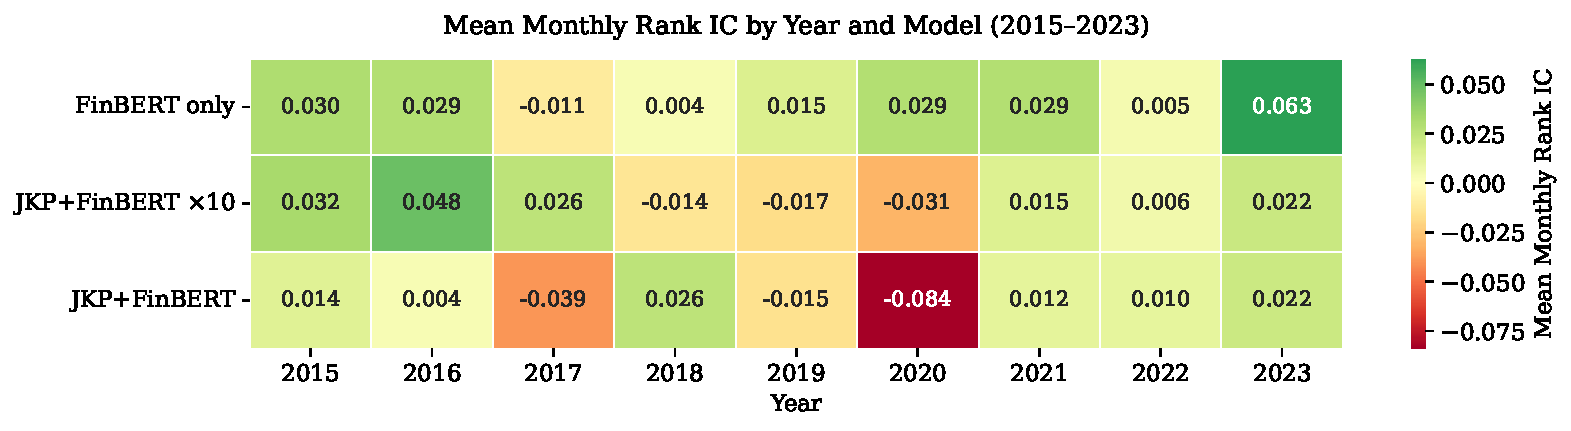
\includegraphics[width=\linewidth]{figures/fig4_ic_heatmap.pdf}
    \caption{Mean monthly Rank IC by year and model. FinBERT-only (top row)
    is positive in 8 of 9 years.}
    \label{fig:ic_heatmap}
\end{figure}

\begin{table}[H]
\centering
\caption{Rolling-window summary over 108 out-of-sample months (2015--2023).}
\label{tab:rolling}
\begin{tabular}{lrrrr}
\toprule
\textbf{Model} & \textbf{Mean IC} & \textbf{\% IC $>0$} & \textbf{IC $t$-stat} &
\textbf{Roll-12M net} \\
\midrule
\textbf{FinBERT only}      & $\mathbf{0.0214}$ & $\mathbf{62\%}$ & $\mathbf{2.67}$ & $\mathbf{+6.75\%}$ \\
JKP only                   & NaN  & --- & --- & $-7.20\%$ \\
JKP + FinBERT              & $-0.003$ & $23\%$ & $-0.24$ & $-4.74\%$ \\
JKP + FinBERT $\times$10   & $0.010$  & $56\%$ & $1.23$  & $+0.78\%$ \\
\bottomrule
\end{tabular}
\end{table}

The FinBERT-only model is the \textbf{only statistically significant predictor},
with IC t-statistic $= 2.67$ ($p < 0.01$) across 108 months.
Positive IC in 62\% of months with a stable cross-year pattern
(Figure~\ref{fig:ic_heatmap}) confirms a genuine, persistent cross-sectional signal.

Figure~\ref{fig:rolling} shows the rolling 12-month net return.

\begin{figure}[H]
    \centering
    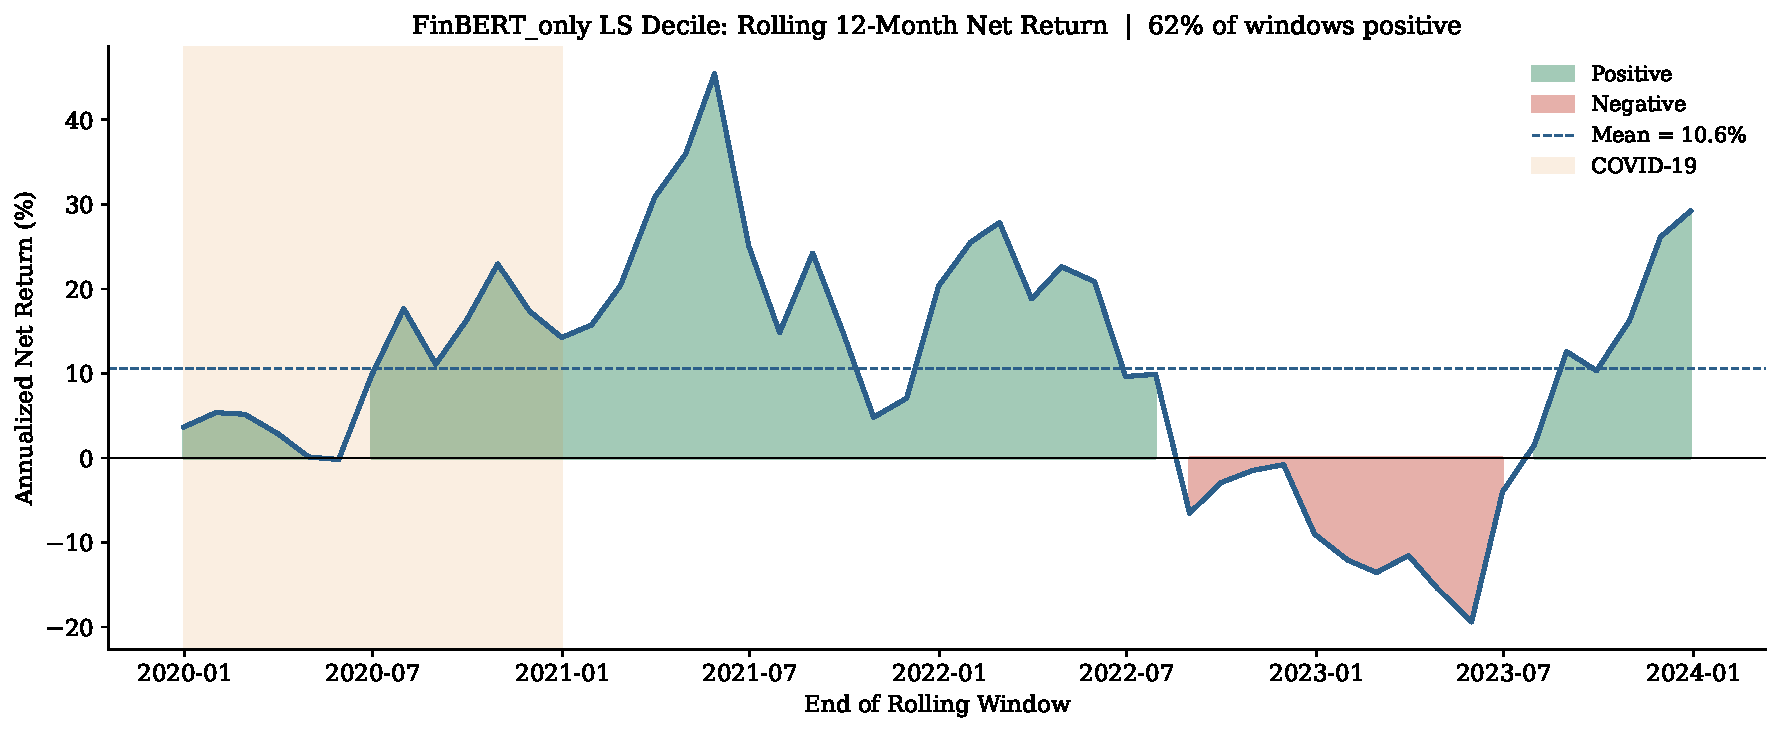
\includegraphics[width=\linewidth]{figures/fig6_rolling_12m.pdf}
    \caption{Rolling 12-month annualised net return for the FinBERT-only LS Decile
    strategy (2019--2023). Mean $= +6.75\%$.}
    \label{fig:rolling}
\end{figure}

% ==============================================================
\section{Discussion}
\label{sec:disc}

\paragraph{Cross-sectional vs.\ time-series signals.}
A central finding is the divergence between Rank IC and backtest performance
for the JKP-containing models.
JKP factors carry the same value for all stocks in a given month; they encode
\textit{market-level} information (business cycle, risk premia).
An XGBoost model trained on these features learns to predict which months are
``good'' versus ``bad'' on average --- market timing.
Evaluated globally, this inflates Rank IC (high temporal correlation).
But in portfolio construction, where returns are long minus short
\textit{within} each month, a constant prediction within any month produces
a random portfolio.
This explains why JKP-only yields undefined monthly Rank IC and negative net backtest
returns after transaction costs.

In contrast, FinBERT sentiment varies \textit{across firms} in the same month,
providing genuine cross-sectional discrimination.

\paragraph{The combination paradox.}
Adding JKP features to FinBERT \textit{reduces} out-of-sample net performance.
We attribute this to two mechanisms: (1) XGBoost allocates split budget to
high-gain JKP features that are time-series predictors, crowding out FinBERT
splits; (2) the higher turnover of JKP-driven portfolios (91\% vs.\ 58\%)
generates 3--4\% additional annual cost drag.
The feature-weighting approach ($\times$10) partially recovers global Rank IC
but fails in practice, suggesting that the improved IC reflects time-series
variance rather than improved cross-sectional discrimination.

\paragraph{Limitations.}
\begin{enumerate}[noitemsep]
    \item \textbf{Universe bias}: the freshness filter retains only firms with
          recent earnings calls (typically mid- and large-caps).
          Results may not generalise to small firms.
    \item \textbf{Test period length}: five years (2019--2023) is short for
          definitive inference; our 108-month rolling analysis partially mitigates this.
    \item \textbf{Transaction costs}: 0.2\% one-way is conservative for large-caps
          but may underestimate costs for smaller firms in our universe.
    \item \textbf{FinBERT context window}: the 512-token limit requires text
          chunking; very long transcripts lose information beyond the first
          few thousand tokens.
\end{enumerate}

% ==============================================================
\section{Conclusion}

We demonstrate that fresh earnings-call sentiment, engineered with
quarter-over-quarter delta features and cross-sectional standardisation,
provides a statistically significant and economically meaningful cross-sectional
signal for excess stock returns.

Our key contributions are:
\begin{itemize}[noitemsep]
    \item A \textbf{freshness filter} ($\leq 3$ months) that eliminates stale signals
          and recovers predictive power absent in the raw unfiltered data.
    \item A \textbf{structural diagnosis} of JKP factors: their within-month
          constancy makes them time-series rather than cross-sectional predictors.
    \item A \textbf{robust out-of-sample evaluation} spanning 108 months with
          explicit transaction costs, multi-period breakdowns, and a formal
          t-test on the Rank IC ($t = 2.67$).
\end{itemize}

The FinBERT-only long-short decile strategy delivers $+11.4\%$ net annualised
return and a Sharpe ratio of 0.79 over the 2019--2023 test period, with
consistent positive performance across all three sub-periods (pre-COVID,
COVID, post-COVID).

% ==============================================================
\bibliographystyle{plainnat}
\begin{thebibliography}{9}

\bibitem[Araci(2019)]{araci2019}
Araci, D. (2019).
\newblock FinBERT: Financial Sentiment Analysis with Pre-trained Language Models.
\newblock \textit{arXiv preprint arXiv:1908.10063}.

\bibitem[Grinold \& Kahn(1999)]{grinold1999}
Grinold, R.~C. and Kahn, R.~N. (1999).
\newblock \textit{Active Portfolio Management}.
\newblock McGraw-Hill, 2nd edition.

\bibitem[Huang et al.(2023)]{huang2023}
Huang, A.~H., Zang, A.~Y., and Zheng, R. (2023).
\newblock Evidence on the Information Content of Text in Analyst Reports.
\newblock \textit{Journal of Financial Economics}, 147(1), 1--28.

\bibitem[Jensen, Kelly \& Pedersen(2023)]{jkp2023}
Jensen, T.~I., Kelly, B.~T., and Pedersen, L.~H. (2023).
\newblock Is There a Replication Crisis in Finance?
\newblock \textit{Journal of Finance}, 78(5), 2465--2518.

\end{thebibliography}

\end{document}
